\documentclass{jknotes}
\usepackage{../joshkirklin}

\tikzset{
    partial ellipse/.style args={#1:#2:#3}{
        insert path={+ (#1:#3) arc (#1:#2:#3)}
    }
}

\setmathfont{Latin Modern Math}
\setmathfont{GFS NeoHellenic Math}[range=bfsfup/{greek,Greek}->it]
\setmathfont{GFS NeoHellenic Math}[range=sfup/{latin,Latin}->it]
\newcommand{\Ra}{\text{Ra}}

\usetikzlibrary{intersections, pgfplots.fillbetween}
\begin{document}

\institution{Cambridge Part III Maths}
\title{Fluid Dynamics of the Solid Earth}
\lecturer{Dr. Jerome Neufeld}
\notetaker{Charles Powell}
\date{Lent 2020}

\maketitle
\suggestionsspiel
\tableofcontents

\lecture{21/01/21}
\section{Introduction}
The course will use the wealth of observations of the solid Earth to motivate
mathematical models of the physical processes governing its evolution. The
dynamic evolution is governed by a rich variety of physical processes occuring
on a wide range of length and time scales. 

\begin{itemize}
	\item The Earth's core is formed by the solidifcation of a mixture of
		molten iron and various light elements, a process which drives
		predominantly compositional convection in the liquid outer core, thus
		producing the geodynamo responsible for the Earth's magnetic field. 
	\item On million year timescales, the solid mantle convects, and as it
		upwells to the surface it partially melts leading to the volcanism. 
	\item At the surface, convection drives the motion of brittle plates which
		are responsible for the Earth's topography as can be felt and imaged
		through the seismic record (figure~\ref{fig:seismology})
	\item In the Earth's surface, fluids flow through porous rocks, for
		example groundwater aquifers which feed streams and rivers which erode
		the solid surface.
	\item On the Earth's surface, similar physical processes of viscous and
		elastic deformation coupled to phase changes govern the evolution of
		the Earth's cryosphere, from the solidification of sea ice to the flow
		of glacial ice over land and ice shelves over the ocean.
\end{itemize}
\begin{figure}
	\centering
	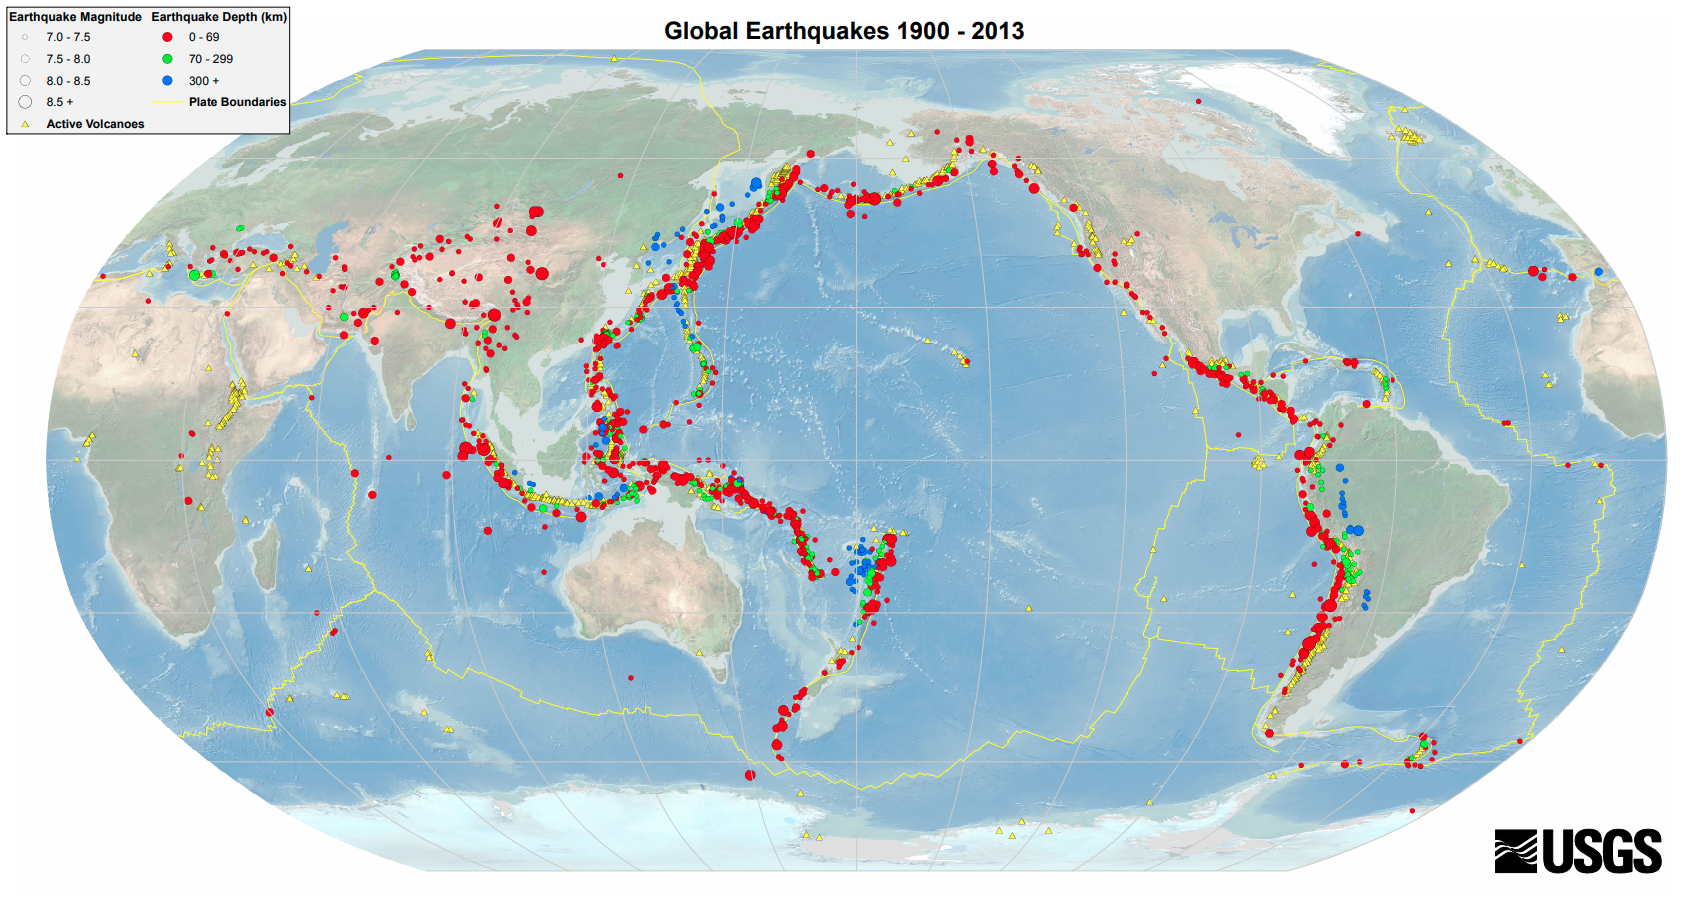
\includegraphics[width=\textwidth]{earthquakes.png}
	\caption{Map of global earthquakes, visibly localised to tectonic plate
	boundaries.}
	\label{fig:seismology}
\end{figure}

Predominantly, the mathematics is of slow viscous flows. Topics include the
onset and scaling of convection, the coupling of fluid motions with changes of
phase at a boundary, the thermodynamic and mechanical evolution of
multicomponent or multiphase systems, the coupling of fluid flow and elastic
flexure or deformation, and the flow of fluids through porous materials. 

\section{Plate cooling}
Here we consider a half-space cooling model of the oceanic lithosphere
(oceanic plates). The bottom surface of Earth's oceans, particularly clear in
the Atlantic ocean, has a large scale structure in which the middle of the
ocean (the \emph{mid-ocean ridge}) is shallower than regions closer to the
continents.  The mid-ocean ridge forms as a result of separating tectonic
plates. We know that the plates move apart here due to magnetic anomalies
forming `stripes' of alternating polarity. The quasi-periodic flipping of the
Earth's magnetic polarity allows dating of the stripes. The plates are driven
apart by convection of the Earth's mantle.

\subsection{Thermal  problem}
We wish to form a model describing the depth of the ocean floor near mid-ocean
ridges. First we estimate the temperature field. Consider an idealised model
with a flat surface (for now), observed plate spreading rate $U$, surface
temperature $T_0$, deep mantle temperature $T_1$.
The temperature field is described by the advection-diffusion equation
\begin{equation}
	\rho c_p \left(\frac{\partial T}{\partial t} + \symbf{u}\cdot\nabla T
	\right) = \nabla \cdot (k \nabla T)
\end{equation}
where $c_p$ is specific heat capacity, $k$ is thermal conductivity, $\rho$ is
density, all assumed constant. For simplicity, we combine these constants into
the thermal diffusivity $\kappa = k/\rho c_p$. Then
\begin{equation}
	\frac{\partial T}{\partial t} + \symbf{u}\cdot\nabla T
	 = \kappa \nabla^2 T
\end{equation}

\begin{figure}
	\begin{center}
	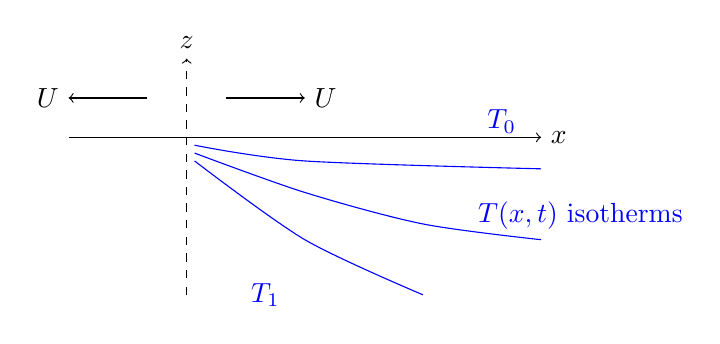
\begin{tikzpicture}
		\draw[->] (-3, 0) -- (3, 0) node[right] {$x$};
		\draw[dashed,->] (-1.5, -2) -- (-1.5, 1) node[above] {$z$};
		\draw[->] (-1, 0.5) -- (0, 0.5) node[right] {$U$};
		\draw[->] (-2, 0.5) -- (-3, 0.5) node[left] {$U$};
		\draw[smooth,blue] plot coordinates {(-1.4, -0.1) (0, -0.3) (3,
		-0.4)};
		\draw[smooth,blue] plot coordinates {(-1.4, -0.2) (0, -0.7) (1.5,
			-1.1) (3, -1.3)};
		\draw[smooth,blue] plot coordinates {(-1.4, -0.3) (0, -1.3) (1.5,
		-2)};
		\draw[blue] (3.5, -1) node {$T(x,t)$ isotherms};
		\draw[blue] (2.5, 0.2) node {$T_0$};
		\draw[blue] (-0.5, -2) node {$T_1$};
	\end{tikzpicture}
	\caption{Schematic diagram of mid-ocean ridge spreading and mantle
	temperature isotherms.}
\end{center}
\end{figure}


We wish to find the steady state profile with $\partial_t = 0, \symbf{u} = U
\hat{\symbf{x}}$ where $U$ is constant. Note that far from the ridge axis, the
thickness of the plate is much smaller than the extent of the plate. Hence in
terms of scalings, $z \ll x$ and we may neglect the $\partial_x^2$ component
of $\nabla^2$. We have
\begin{equation}
	U \frac{\partial T}{\partial x} = \kappa \left( \frac{\partial^2
	T}{\partial x^2} + \frac{\partial^2 T}{\partial z^2}\right) \approx \kappa
	\frac{\partial^2 T}{\partial z^2}
	\label{eq:temp}
\end{equation}
The scaling given by this equation is $U\Delta T / x \sim \kappa \Delta T /
z^2$ where $\Delta T = T_1 - T_0$ is the natural temperature scale. There is
no natural lengthscale, so we use that given by the advection-diffusion
equation:
\begin{equation}
	z \sim \sqrt{\frac{\kappa x}{U}}
\end{equation}

We can proceed by finding a self-similar solution with similarity variable
\begin{equation}
	\eta = \frac{z}{2\sqrt{\frac{\kappa x}{U}}}
\end{equation}
and seek solutions of the form
\begin{equation}
	\theta = \frac{T - T_0}{T_1-T_0} = \theta(\eta)
\end{equation}
Using the variables $\eta, \theta$, \eqref{eq:temp} becomes
\begin{align}
	-U\Delta T \frac{\eta}{2x} \theta_\eta &= \frac{\kappa \Delta T}{4
	\frac{\kappa x}{U}} \theta_{\eta\eta}\\
		\implies \theta_{\eta\eta} + 2\eta\theta_\eta &= 0
\end{align}
We can integrate directly to get $\theta_\eta = ae^{-\eta^2}$, which gives
\begin{equation}
	\theta = b + a \int_0^\eta e^{-y^2} \, \diffd y
\end{equation}
The boundary conditions are $\theta(0) = 1$ and $\theta(\infty) = 1$ based on
the definitions of $T_0$ and $T_1$. The thermal structure away from the ridge
is then
\begin{equation}
	T = T_0 + (T_1-T_0) \erf\left( \frac{z}{2\sqrt{\frac{\kappa x}{U}}}\right)
	\label{eq:T}
\end{equation}
where the error function $\erf$ and its complement erfc are defined by
\begin{align}
	\erf(x) &= \frac{2}{\sqrt{\pi}} \int_0^x e^{-y^2} \, \diffd y \\
	\text{erfc}(x) &= 1 - \erf(x)
\end{align}

\subsection{Ocean depth away from mid-ocean ridge}
We now consider the depth of the ocean following from the temperature field
derived above. We choose axes with $z$ increasing downwards, placing the sea
surface at $z=0$ and the `bottom' of the mantle at $z=H$. The coordinate $x$
increases away from the mid-ocean ridge, with ocean depth $w(x)$ at a given
$x$.

\begin{figure}
	\begin{center}
	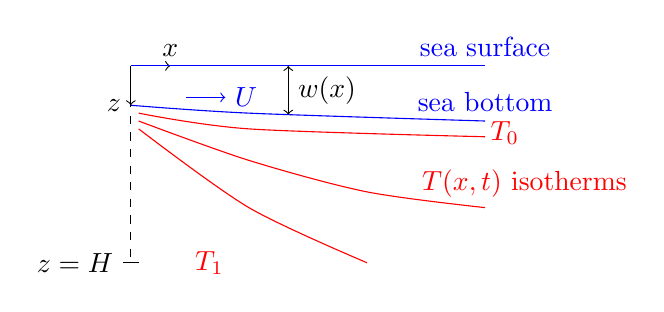
\begin{tikzpicture}
		\draw[->] (-1.5, 0.5) -- (-1.5, 0) node[left] {$z$};
		\draw[->] (-1.5, 0.5) -- (-1, 0.5) node[above] {$x$};
		\draw[dashed] (-1.5, 0.5) -- (-1.5, -2);

		\draw[blue,->] (-0.8, 0.1) -- (-0.3, 0.1) node[right] {$U$};
		\draw[blue] (-1.5, 0.5) -- (3, 0.5) node[above] {sea surface};

		\draw[smooth,red] plot coordinates {(-1.4, -0.1) (0, -0.3) (3,
		-0.4)};
		\draw[smooth,red] plot coordinates {(-1.4, -0.2) (0, -0.7) (1.5,
			-1.1) (3, -1.3)};
		\draw[smooth,red] plot coordinates {(-1.4, -0.3) (0, -1.3) (1.5,
		-2)};
		\draw[red] (3.5, -1) node {$T(x,t)$ isotherms};
		\draw[red] (3.25, -0.35) node {$T_0$};
		\draw[red] (-0.5, -2) node {$T_1$};

		\draw[smooth,blue] plot coordinates {(-1.5,0) (0, -0.1) (3, -0.2)};
		\draw[blue] (3, -0.2) node[above] {sea bottom};

		\draw[<->] (0.5, 0.5) -- (0.5, -0.12) node[midway,right] {$w(x)$};
		\draw (-1.4, -2) -- (-1.6, -2) node[left] {$z=H$};
	\end{tikzpicture}
	\caption{Schematic diagram of ocean depth and crust temperature surfaces.}
\end{center}
\end{figure}

First, consider \emph{isostacy}: Archimedean buoyancy applied
to Earth's crust. This indicates the depth at which an object/fluid parcel of some 
density lies in a fluid of different density. 
\begin{center}
	\begin{tikzpicture}[scale=2]
		\draw[blue] (-2, 0) -- (-1, 0); 
		\draw (-1, 0.3) -- (1, 0.3) -- (1, -0.3) -- (-1,
		-0.3) -- (-1, 0.3);
		\draw[blue] (1, 0) -- (2, 0);
		\draw[<->] (0.5, 0.3) -- (0.5, -0.3) node[midway,right] {$h$};
		\draw (-0.5, 0) node {$\rho_c$};
		\draw (-1.5, -0.3) node {$\rho_m$};
		\draw[<->] (1.2, 0) -- (1.2, -0.3) node[midway, right] {$b$};
	\end{tikzpicture}
\end{center}
Denoting the density of the crust and mantle as $\rho_c, \rho_m$ respectively,
the crust of thicknes $h$ sits at a depth $b$ in the mantle. Hydrostatic
balance gives $\rho_c g h = \rho_m g b$. Equivalently, we can consider a force
balance between the weight of the curst and the buoyancy force:
\begin{equation}
	\rho_c (h-b) g = (\rho_m - \rho_c) gb
\end{equation}

Within the oceanic lithosphere we have a denssity field
\begin{equation}
	\rho = \rho_m \left( 1- \alpha (T - T_1)\right)
\end{equation}
where $T=T(x,z)$ is the thermal model derived above, given by \eqref{eq:T}.
Isostatic balance gives the following, which balances water weight, mantle
weight, with water and mantle buoyancy. The ocean density is denoted by
$\rho_w$.

\begin{align}
	\rho_w w_0 + \rho_m (H - w_0) &= \rho_w w(x) + \int_w^H \rho(T) \, \diffd
	z \\
	  &= \rho_w w + \rho_m (H-w) - \rho_m \alpha \int_w^H (T-T_1) \, \diffd z \\
	\implies (\rho_m - \rho_w)(w-w_0) &= - \rho_m \alpha \int_w^H (T-T_1) \,
	\diffd z \\
	&\approx  - \rho_m \alpha (T_1 - T_0) \int_0^\infty \text{erfc}(\eta)
	\cdot 2 \sqrt{\frac{\kappa x}{U}} \, \diffd \eta
\end{align}
where the last approximate equality follows from taking $w \to 0$ and $H \to
\infty$, approximating the fact the mantle is much deeper than the ocean. The
ocean depth is therefore
\begin{equation}
	w-w_0 = \frac{\rho_m}{\rho_m - \rho_w} \alpha (T_1-T_0)
	\frac{2}{\sqrt{\pi}} \left(\frac{\kappa x}{U}\right)^{1/2}
\end{equation}
This model fits the data well near to the mid-ocean ridge, with crust age up
to 75 million years. However, away from the ridge, the model breaks down as
$w$ tends to a constant as $x \to \infty$. The breakdown of the model is due
to convection: the infinite depth curst approximation breaks down and
convection dynamics become important.

\section{Natural convection}
Natural convection arises in flows driven by density differences in a
gravitational field, e.g. due to temperature or composition.

\subsection{Static stability}
Consider the case of no fluid motion $\symbf{u} = 0$ and initial
stratification $\rho = \rho_0 (1+\beta z)$.  If $\beta < 0$, the dynamics are
statically stable. If $\beta > 0$, the dynamics are statically unstable but
dynamically could be stable. 

\begin{center}
	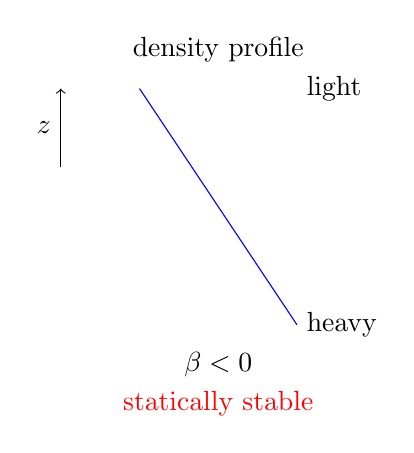
\begin{tikzpicture}
		\draw[blue] (0,0) -- (2, -3);
		\draw (2, 0) node[right] {light};
		\draw (2, -3) node[right] {heavy};

		\draw[->] (-1, -1) -- (-1, 0) node [midway,left] {$z$};
		\draw (1, -3.5) node {$\beta < 0$};
		\draw (1, 0.5) node {density profile};
		\draw[red] (1, -4) node {statically stable};
	\end{tikzpicture}
	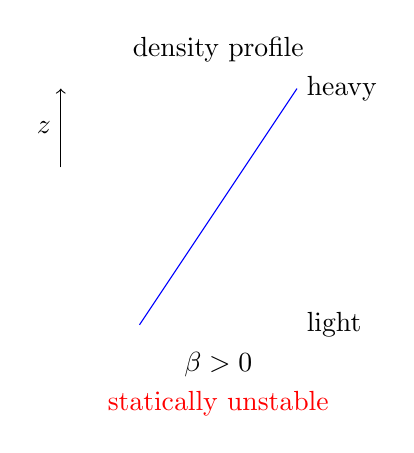
\begin{tikzpicture}
		\draw[blue] (2,0) -- (0, -3);
		\draw (2, -3) node[right] {light};
		\draw (2, 0) node[right] {heavy};

		\draw[->] (-1, -1) -- (-1, 0) node [midway,left] {$z$};
		\draw (1, -3.5) node {$\beta > 0$};
		\draw (1, 0.5) node {density profile};
		\draw[red] (1, -4) node {statically unstable};
	\end{tikzpicture}
\end{center}

\paragraph{Scaling analysis.} Consider a fluid parcel of characteristic size
$l$ in unstable density profile $\rho = \rho_0 (1+\beta z), \beta > 0$.
Suppose the parcel moves up a distance $h$ in time $\tau$.
\begin{center}
	\begin{tikzpicture}
		\draw[blue] (2,0) -- (0, -3);
		\draw (0.7, -3+0.7*3/2) circle (0.2);
		\draw[<->] (1, -2.15) -- (1, -1.75) node[midway,right] {$l$};
		\draw[dashed] (0.7, -1) circle (0.2);
		\draw[<->] (0.3, -3+0.7*3/2) -- (0.3, -1) node[midway,left] {$h$};
		\draw[blue] (2,0) node[right] {$\rho = \rho_0 (1+\beta z)$};
	\end{tikzpicture}
\end{center}

The rise of the fluid parcel relasess potential energy $E$ which scales as
\begin{equation}
	E \sim (\Delta \rho l^3) g h \sim (\rho_0 \beta h l^3) g h \sim \rho_0
	\beta g h^2 l^3
\end{equation}
The timescale for the rising motion is limited by diffusion of buoyancy (i.e.
diffusion of temperature in this case) so $\tau \sim l^2/\kappa$ where
$\kappa$ is thermal diffusivity. Viscous dissipation over timescale $\tau$
scales as the shear stress times the distance travelled:
\begin{equation}
	\mathcal{D} \sim \frac{\mu U}{l}l^2 h \sim \mu \frac{h/\tau}{l} l^2 h \sim
	\frac{\mu \kappa h^2}{l}
\end{equation}

Instability arises if $E \gtrapprox \mathcal{D}$, which we can write as
\begin{equation}
	\rho_0 \beta g h^2 l^3 \gtrapprox \frac{\mu \kappa h^2}{l}
\end{equation}
Define the \emph{Rayleigh number}
\begin{equation}
	\text{Ra} = \frac{\rho_0 \beta g l^4}{\kappa \mu}
\end{equation}
which quantifies the ratio of timescales of thermal transport via diffusion
versus via convection. If $\text{Ra}$ is large, the flow is more turbulent.
There is instability if $\text{Ra} \gtrapprox \mathcal{O}(1)$.

\subsection{Onset of convection}
Consider a fluid of depth $h$ between $z=0$ and $z=h$ with density profile
$\rho(z)$ and temperature difference $\Delta T$ across the depth.

\begin{center}
	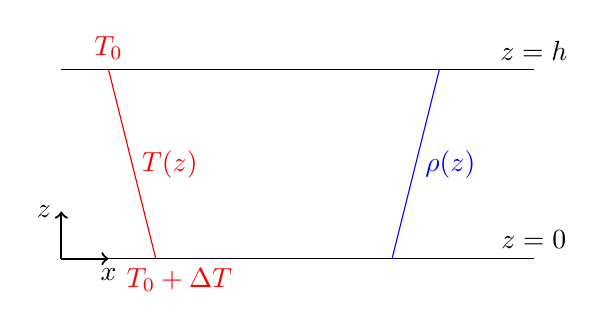
\begin{tikzpicture}[scale=1.2]
		\draw  (0, 2) -- (5, 2);
		\draw (0, 0) -- (5, 0);
		\draw[thick,->] (0, 0) -- (0.5, 0) node[below] {$x$};
		\draw[thick,->] (0, 0) -- (0, 0.5) node[left] {$z$};
		\draw (5, 0.2) node {$z=0$};
		\draw (5, 2.2) node {$z=h$};
		\draw[red] (0.5, 2) -- (1, 0) node[midway,right] {$T(z)$};
		\draw[red] (0.5, 2) node[above] {$T_0$};
		\draw[red] (1.25, 0) node[below] {$T_0 + \Delta T$};
		\draw[blue] (3.5,0) -- (4, 2) node[midway,right] {$\rho(z)$};
	\end{tikzpicture}
\end{center}

The governing equations are conservation of mass \eqref{eq:masscons},
conservation of momentum \eqref{eq:momcons}, and conservation of energy
\eqref{eq:energycons}.
\begin{align}
	\nabla \cdot \symbf{u} &= 0 \label{eq:masscons} \\
	\rho \left( \frac{\partial \symbf{u}}{\partial t} +
	\symbf{u}\cdot\nabla\symbf{u}\right) &= - \nabla p + \mu \nabla^2
	\symbf{u} - \rho g \hat{\symbf{z}} \label{eq:momcons} \\
	\rho c_p \left( \frac{\partial T}{\partial t} + \symbf{u} \cdot \nabla T
	\right) &= \nabla \cdot (k \nabla T) \label{eq:energycons}
\end{align}

For steady solutions with $\symbf{u} = 0$ and $\partial_t = 0$ we find
\begin{align}
	T &= T_0 + \Delta T \left(1-\frac{z}{h}\right) \\
	\frac{\partial p}{\partial x} = \frac{\partial p}{\partial y} &= 0 \\
	\frac{\partial p}{\partial z} &= - \rho_0 g \left( 1- \alpha
	(T-T_0)\right) 
\end{align}
We assess the stability by examining small perturbations to a steady base
state:
\begin{align}
	\symbf{u} &= 0 + \symbf{u}'(\symbf{x},t) \\
	T &= T_0 + \Delta T \left(1-\frac{z}{h}\right) + T'(\symbf{x},t) \\
	p &= p_0(z) + p'(\symbf{x},t) 
\end{align}
The linearied perturbation equations are thus
\begin{align}
	\nabla \cdot \symbf{u}' &= 0  \\
	\rho_0  \frac{\partial \symbf{u}'}{\partial t} &= - \nabla p' + \mu
	\nabla^2 \symbf{u}' + \rho_0 g \alpha T' \hat{\symbf{z}} \\
	\frac{\partial T'}{\partial t} - \frac{\Delta T}{h} w' &= \kappa \nabla^2
	T'
\end{align}

\paragraph{Non-dimensionalising.}
We wish to non-dimensionalise these equations. There are two intrinsic
scales, temperature $\sim \Delta T$ and lengths $\sim h$. We form velocity and
time characteristic scales via \emph{diffusive scaling}. From the thermal
equation:
\begin{equation}
	\frac{\Delta T}{t} \sim \frac{\Delta T U}{h} \sim \frac{\kappa \Delta
	T}{h^2}
\end{equation}
From the second relation we have $U \sim \kappa/h$, then from the first we
have $t \sim h^2/\kappa$.  The non-dimensionalised equations (dropping $'$
henceforth) are
\begin{align}
	\nabla \cdot \symbf{u} &= 0 \label{eq:L2:1}\\
	\frac{1}{\text{Pr}} \frac{\partial \symbf{u}}{\partial t} &= - \nabla p +
	\nabla^2 \symbf{u} + \text{Ra}T \hat{\symbf{z}} \label{eq:L2:2}\\
	\frac{\partial T}{\partial  t} - w &= \nabla^2 T  \label{eq:L2:3}
\end{align}
where the \emph{Prandtl number} $\text{Pr} = \frac{\mu/\rho_0}{\kappa}$ which
quantifies the importance of viscous diffusion versus thermal diffusion.

\paragraph{Boundary conditions.} We require boundary conditions on the
temperature $T$ and velocity $\symbf{u}$. There are several possible
conditions, which may be mixed:
\begin{itemize}
	\item Rigid boundary $\left[ \symbf{u}\cdot\hat{\symbf{n}}
		\right]_{\text{boundary}} = 0$ where $\hat{\symbf{n}}$ is outwards
		normal of boundary surface
	\item	No-slip $\left[ \symbf{u}\times\hat{\symbf{n}}
		\right]_{\text{boundary}} = 0$
	\item Stress-free (free slip) $\mu\frac{\partial u}{\partial n} = \mu
		\frac{\partial v}{\partial n} = 0$ i.e. $n=z$ in our picture
	\item Fixed temperature $T_{\text{boundary}} = \text{const.}$
	\item Fixed heat flux $\left[ \hat{\symbf{n}}\cdot\nabla
				T\right]_{\text{boundary}} = \text{const.}$
\end{itemize}

We eliminate pressure from the non-dimensionalised equations by taking
$\hat{\symbf{z}}\cdot\nabla \times (\nabla \times \eqref{eq:L2:2}$. Recall the
vector identity
\begin{equation}
	\nabla \times (\nabla \times \symbf{A}) = \nabla (\nabla \cdot \symbf{A})
	- \nabla^2 \symbf{A}
\end{equation}
The governing equations are reduced to
\begin{align}
	\left( \text{Pr}^{-1} \partial_t - \nabla^2 \right) \nabla^2 w &=
	\text{Ra} \nabla^2_H T \label{eq:L2:4}\\
	\left( \partial_t - \nabla^2 \right) T &= w \label{eq:L2:5}
\end{align}
where $\nabla_H = (\partial_x, \partial_y, 0)$ is the horizontal gradient.

\paragraph{Normal modes.} We examine growth/decay of perturbations of the form
\begin{equation}
	(w,T) = (\hat{w}(z),\hat{T}(z))e^{i(kx+ly)+\sigma t}
\end{equation}
For convenience, and given the $x, y$ symmetry, define $a^2 = k^2 + l^2$ as an
effective horizontal wavenumber. We have from the governing equations
\eqref{eq:L2:4}, \eqref{eq:L2:5}:
\begin{align}
	\left[\sigma \text{Pr}^{-1} - (D^2 - a^2)\right](D^2-a^2) &= -\text{Ra}
	a^2 \hat{T} \label{eq:L2:6}\\
	\left[ \sigma - (D^2 - a^2) \right] \hat{T} &= \hat{w} \label{eq:L2:7}
\end{align}
where $D = \diffd/\diffd z$. The boundary in our case will be
rigid, stress free, and fixed temperature. Note that this is not necessarily
representative of the actual boundary conditions, but is useeful analytically.
 Thus at $z= 0, 1$ we have $w = 0$ (rigid), $D^2 w = 0$ (stress free) and $T=
 0 $ (fixed temperature). Given these conditions, the heat equation implies
 $D^2 T = 0$ on $z=0,1$ and the momentum equation implies $D^4 w = 0$ on
 $z=0,1$. 

 \paragraph{Marginal stability.} The marginal stability boundary is $\sigma =
 0$ between growth ($\sigma > 0$) and decay ($\sigma < 0$). Combining
 \eqref{eq:L2:6} and \eqref{eq:L2:7} with $\sigma = 0$ we hae
 \begin{equation}
	 (D^2 - a^2)^3 (\hat{T},\hat{w}) = -a^2 \text{Ra}(\hat{T},\hat{w})
 \end{equation}
 The solutions have structure 
 \begin{equation}
	 (\hat{T}, \hat{w}) =  (\hat{T}_0, \hat{w}_0) \sin n \pi z
 \end{equation}
 Hence we have the eigenvalue condition $(n^2 \pi^2 + a^2)^3 = a^2 \text{Ra}$.
 Let $a^2 = \pi^2 b^2$. Then
 \begin{equation}
	 \text{Ra} = \frac{(n^2 + b^2)^3 \pi^4}{b^2}
 \end{equation}

 The minimum Rayleigh number is at $n=1$ where $\text{Ra} = (1+b^2)^3
 \pi^4/b^2$:
 \begin{center}
	 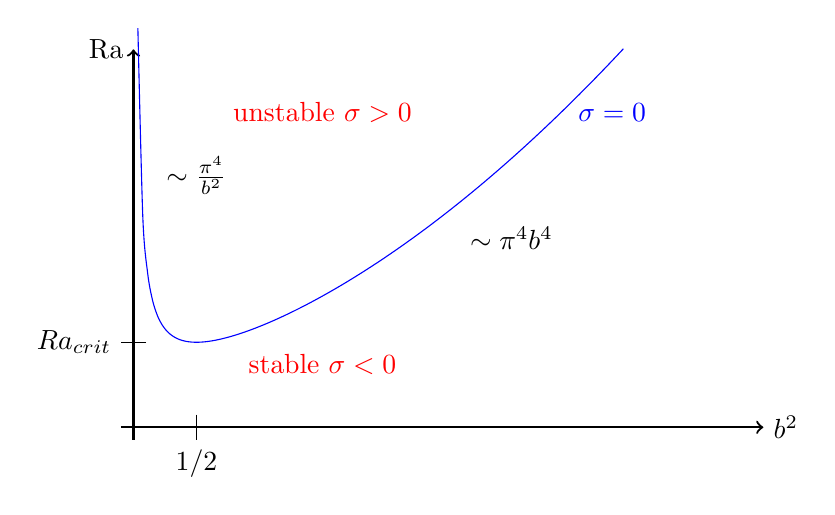
\begin{tikzpicture}[scale=1.6]
		 \draw[thick,->] (-0.1, 0) -- (5, 0) node[right] {$b^2$};
		 \draw[thick,->] (0, -0.1) -- (0, 3) node[left] {Ra};
		 \draw[smooth,blue] plot[domain=0.035:3.89,samples=100]  ({\x},{(1+\x)^3/(10*\x)});
		 \draw (0.5,0.1) -- (0.5, -0.1) node[below] {$1/2$};
		 \draw (0.1, 0.675) -- (-0.1, 0.675) node[left]
		 {$\text{Ra}_{\text{crit}}$};
		\draw (0.5, 2) node {$\sim \frac{\pi^4}{b^2}$};
		\draw (3, 1.5) node {$\sim \pi^4 b^4$};
		\draw[blue] (3.8, 2.5) node {$\sigma = 0$};
		\draw[red] (1.5, 0.5) node {stable $\sigma < 0$};
		\draw[red] (1.5, 2.5) node {unstable $\sigma > 0$};
	 \end{tikzpicture}
 \end{center}

 Setting $\partial \text{Ra}/\partial b^2 = 0$ to find the critical Rayleigh
 number $\text{Ra}_{\text{crit}}$, we find
 \begin{equation}
	 \text{Ra}_{\text{crit}} = \frac{27 \pi^4}{4} \approx 657.5 \hspace{2em}
	 \text{at}\,\,\, a = \frac{\pi}{\sqrt{2}}
 \end{equation}
Hence the dimensional wavelength at critical Rayleigh number is $2\pi h/a =
2\sqrt{2} h \approx 2.8 h$. The convection process appears like so:
\begin{center}
	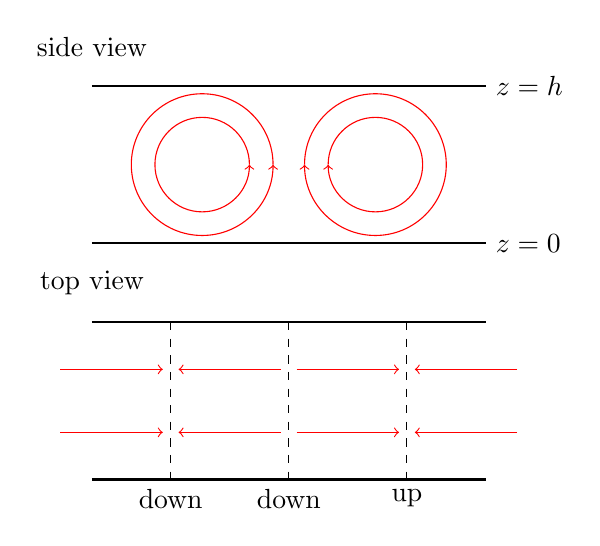
\begin{tikzpicture}
		\draw (0, 2.5) node {side view};
		\draw[thick] (0,0) -- (5, 0) node[right] {$z=0$};
		\draw[thick] (0,2) -- (5, 2) node[right] {$z=h$};
		\draw[red,->] (2.3, 1) arc(0:360:0.9);
		\draw[red,<-] (2.7, 1) arc(-180:180:0.9);
		\draw[red,->] (2.0, 1) arc(0:360:0.6);
		\draw[red,<-] (3.0, 1) arc(-180:180:0.6);
	\begin{scope}[shift={(0,-3)}]
		\draw (0, 2.5) node {top view};
		\draw[thick] (0,0) -- (5, 0);
		\draw[thick] (0,2) -- (5, 2);
		\draw[dashed] (1, 2) -- (1, 0) node[below] {down};
		\draw[dashed] (4, 2) -- (4, 0) node[below] {up};
		\draw[dashed] (2.5, 2) -- (2.5, 0) node[below] {down};
		\draw[red,->] (2.6, 0.6) -- (3.9, 0.6);
		\draw[red,->] (2.6, 1.4) -- (3.9, 1.4);
		\draw[red,->] (2.4, 0.6) -- (1.1, 0.6);
		\draw[red,->] (2.4, 1.4) -- (1.1, 1.4);
		\draw[red,->] (-0.4, 0.6) -- (0.9, 0.6);
		\draw[red,->] (-0.4, 1.4) -- (0.9, 1.4);
		\draw[red,->] (5.4, 0.6) -- (4.1, 0.6);
		\draw[red,->] (5.4, 1.4) -- (4.1, 1.4);
	\end{scope}
	\end{tikzpicture}
\end{center}

\begin{eg}
	\textbf{Mantle convection.} In the mantle, internal heating is due to
	radiogenic decay. We model this by adding a source term to the conservation of
	energy equation:
	\begin{equation}
		\rho_0 c_p \left( \frac{\partial T}{\partial t} + \symbf{u}\cdot\nabla
		T\right) = \nabla \cdot (k\nabla T) + \rho_0 Q
	\end{equation}
	where $Q = 10^{11} \text{W} \text{kg}^{-1}$. The thermal boundary conditions
	are $T(0) = T_s$, i.e. fixed surface temperature, and $\partial T / \partial
	z = 0$ at $z=h$, i.e. zero basal heat flux.

	A scaling analysis gives 
	\begin{equation}
		x \sim h, \frac{k \Delta T}{h^2} \sim \rho_0 Q
		\implies \Delta T \sim \frac{\rho_0 Q h^2}{k}
	\end{equation}
	The Rayleigh number in this case is
	\begin{equation}
		\text{Ra}_Q = \frac{\rho_0 g \alpha (\rho_0 Q h^2 / k) h^3}{\kappa \mu} =
		\frac{\rho_0^2 g \alpha Q h^5}{k \kappa \mu}
	\end{equation}
	Typical values are $\text{Ra}_Q = 3 \times 10^9$ and $\text{Pr} = 10^{22}$.
	Note that $\text{Ra}_Q$ is much larger than $\text{Ra}_{\text{crit}}$.
\end{eg}

\subsection{High Rayleigh number convection}
At high Rayleigh number, the key idea is: small plumes are generated at
boundaries, which only `see' the statistically well-mixed interior
temperature. Hence heat flux is independent of depth of domain.
\begin{center}
	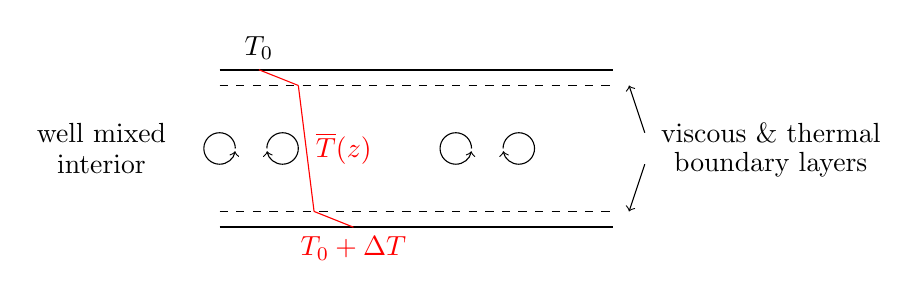
\begin{tikzpicture}
		\draw[thick] (0,0) -- (5, 0);
		\draw[thick] (0, 2) -- (5, 2);
		\draw[dashed] (0, 0.2) -- (5, 0.2);
		\draw[dashed] (0, 1.8) -- (5, 1.8);
		\draw (0.5, 2) node[above] {$T_0$};
		\draw[red] (0.5, 2) -- (1, 1.8);
		\draw[red] (1, 1.8) -- (1.2, 0.2) node[midway,right]
		{$\overline{T}(z)$};
		\draw[red] (1.2, 0.2) -- (1.7, 0) node[below] {$T_0 + \Delta T$};
		\draw[->] (0.2, 1) arc (0:350:0.2);
		\draw[->] (0.6, 1) arc (180:-170:0.2);
		\draw[->] (3.2, 1) arc (0:350:0.2);
		\draw[->] (3.6, 1) arc (180:-170:0.2);
		\draw (7, 1.2) node {viscous \& thermal};
		\draw (7, 0.8) node {boundary layers};
		\draw[->] (5.4, 1.2) -- (5.2, 1.8);
		\draw[->] (5.4, 0.8) -- (5.2, 0.2);
		\draw (-1.5, 1.2) node {well mixed};
		\draw (-1.5, 0.8) node {interior};
	\end{tikzpicture}
\end{center}

The heat flux is characterised by the \emph{Nusselt number} defined by
\begin{equation}
	\text{Nu} = \frac{F_h}{k \Delta T/h} = f(\text{Ra},\text{Pr})
\end{equation}
where $F_h$ is the heat flux, and $\text{Nu}$ is a function of $\text{Ra},
\text{Pr}$ only. If $F_h$ is not a function of $h$, then we must
have
\begin{align}
	F_h = \frac{k \Delta T}{h} f(\text{Ra},\text{Pr}) &\sim \frac{k \Delta
	T}{h} \text{Ra}^{1/3} \\
	\implies F_h &= \lambda(\text{Pr})k \left( \frac{\rho_0 g
	\alpha}{K\mu}\right)^{1/3} \Delta T^{4/3}
\end{align}
for some function $\lambda$.

\paragraph{Boundary layer analysis.}
The picture was formalised by Lou Howard (1965). We assume the thermal
boundary layer grows diffusively (i.e. slowly) according to
\begin{equation}
	\frac{\partial T}{\partial t} = \kappa \frac{\partial^2 T}{\partial z^2} 
\end{equation}
\begin{center}
	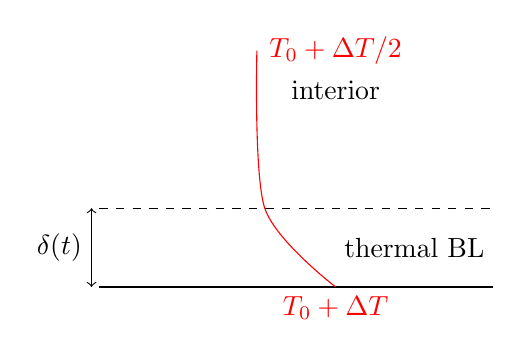
\begin{tikzpicture}
		\draw (0,0) -- (5, 0);
		\draw[dashed] (0,1) -- (5,1);
		\draw[<->] (-0.1, 1) -- (-0.1, 0) node[midway,left] {$\delta(t)$};
		\draw[smooth, red] plot coordinates {(2, 3) (2.1, 1) (3, 0)};
		\draw[red] (3, 3) node {$T_0 + \Delta T /2$};
		\draw (3, 2.5) node {interior};
		\draw (4, 0.5) node {thermal BL};
		\draw[red] (3,0) node[below] {$T_0 + \Delta T$};
	\end{tikzpicture}
\end{center}

Diffusive scaling gives $z \sim \sqrt{\kappa t}$, i.e. a self-similar solution
with similarity variable $\eta = z/2\sqrt{\kappa t}$. The thermal problem can
be solved to get
\begin{equation}
	T = T_0 + \frac{\Delta T}{2}\left[ 1 + \text{erfc}(\frac{z}{2\sqrt{\kappa
	t}})\right]
\end{equation}

The boundary layer is unstable when the local Rayleigh number exceeds the
critical value.
\begin{align}
	\Ra_{BL} = \frac{\rho_0 g \alpha (\Delta T/2) \delta(t)^3}{\kappa \mu}
	&\gtrapprox \Ra_{\text{crit}} \\
	\implies \frac{\delta}{h} &\gtrapprox \left( \frac{2
	\Ra_c}{\Ra}\right)^{1/3}
\end{align}

Assume that advection of plumes from the boundary layer is fast compared with
diffusive growth of the boundary layer. The heat flux is
\begin{equation}
	F_h = \frac{k \Delta T}{2t_c} \int_0^{t_c} \frac{\diffd t}{\sqrt{\pi\kappa
	t}} = \frac{k\Delta T}{\delta_c}
\end{equation}
Hence the Nusselt number can be written
\begin{equation}
	\text{Nu} = \frac{F_h}{k\Delta T/h} = \frac{h}{\delta_c} = \left(
	\frac{\Ra}{2\Ra_c}\right)^{1/3}
\end{equation}
For $\Ra_{\text{crit}} \approx 1100$, the Nusselt number is thus $\text{Nu}
\approx 0.077 \Ra^{1/3}$ which matches well with experiment.

\section{Solidification/melting}.
Applications of solidification/melting theory include
\begin{itemize}
	\item Formation of Earth's crust (early 1800s)
	\item Sea ice, due to Stefan (late 1800s)
	\item Earth's core (mid 1950s)
	\item Igneous rocks (mid 1980s)
\end{itemize}

\subsection{The Stefan condition}
Consider a solid--liquid interface $x = a(t)$ with boundary velocity $v_n$. We
will work in the frame of reference moving with the boundary.
\begin{center}
	\begin{tikzpicture}
		\draw[thick] (0,0) -- (0, 5);
		\draw (2, 1) -- (2, 4) -- (-2, 4) -- (-2, 1) -- (2,1);
		\draw (0,0) node[below] {$x=0$};
		\draw[thick,->] (0, 4.5) -- (1, 4.5) node[right] {$\hat{\symbf{n}}$};
		\draw[->] (2.5, 0.5) -- (1.5, 0.5) node[midway,below] {$v_n$};
		\draw[<-] (-2.5, 0.5) -- (-1.5, 0.5) node[midway,below] {$v_n$};
		\draw[<-] (2.5, 2.5) -- (0.5, 2.5) node[midway,below]
		{$\symbf{q}_l$};
		\draw[->] (-2.5, 2.5) -- (-0.5, 2.5) node[midway,below]
		{$\symbf{q}_s$};
	\end{tikzpicture}
\end{center}

We assume there is a heat flux $\symbf{q}_s$ into the control volume, and a
heat flux $\symbf{q}_l$ leaving the control volume. Assume equal densities for
the liquid and solid, i.e. $\rho_l = \rho_s = \rho$. Conservation of energy in
the control volume gives:
\begin{equation}
	\rho H_l v_n - \hat{\symbf{n}}\cdot\symbf{q}_l - \rho H_s v_n +
	\hat{\symbf{n}} \cdot \symbf{q}_s = 0
\end{equation}
where $\symbf{q} = - k \nabla T$ and $H$ is the \emph{specific enthalpy},
which is the heat energy at constant pressure per unit mass. Rearranging, we
have
\begin{equation}
	\rho (H_l - H_s)v_n = \hat{\symbf{n}}\cdot (\symbf{q}_l - \symbf{q}_s)
\end{equation}
Define $L = H_l - H_s = T_m (s_s - s_l)$ where $T_m$ is the melting
temperature and $s$ is the entropy of solid/liquid. $L$ is the latent heat of
fusion/solidification. At the boundary $x=a(t)$ we have
\begin{equation}
	\rho L v_n = k \hat{\symbf{n}} \cdot (\left.\nabla T \,\right|_s -
	\left.\nabla T \,\right|_l)
\end{equation}
where all quantities are evaluated at the boundary. This is the \emph{Stefan
condition}.

Note that if $\rho_s \ne \rho_l$ there is a velocity $u_n$ induced at the
interface:
\begin{equation}
	u_n = \frac{\rho_l - \rho_s}{\rho_l} v_n
\end{equation}
in which case the Stefan condition is modified to
\begin{equation}
	\rho_s L v_n = k_s \hat{\symbf{n}} \cdot \left.\nabla T \,\right|_s - k_l
	\hat{\symbf{n}} \cdot \left.\nabla T \,\right|_l
\end{equation}

\subsection{1D solification from a cooled boundary}
For convenience we again assume equal densities and thermal properties. 
\begin{center}
	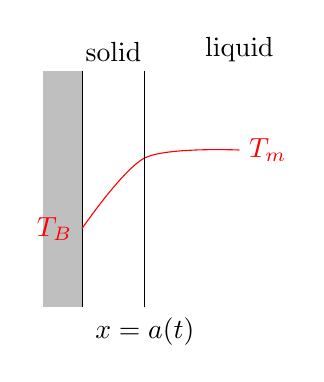
\begin{tikzpicture}
		\draw[thick] (0,0) -- (0, 3);
		\draw[draw=none,fill=gray!50] (0,0) rectangle (-0.5, 3);
		\draw[smooth,red] plot coordinates {(0, 1) (0.8, 1.9) (2, 2)};
		\draw[red] (0, 1) node[left] {$T_B$};
		\draw[red] (2, 2) node[right] {$T_m$};
		\draw (0.8, 0) -- (0.8, 3);
		\draw (0.4, 3) node[above] {solid};
		\draw (2, 3) node[above] {liquid};
		\draw (0.8, 0) node[below] {$x=a(t)$};
	\end{tikzpicture}
\end{center}

In the solid, the temperature $T$ obeys
\begin{equation}
	\frac{\partial T}{\partial t} = \kappa \frac{\partial^2 T}{\partial x^2}
\end{equation}
with boundary conditions $T = T_B$ at $x=0$ and $T = T_m$ at $x= a(t)$. We
also have the Stefan condition
\begin{equation}
	\rho L \dot{a} = k \left.\frac{\partial T}{\partial x} \right|_{a^-}
\end{equation}
at $x = a(t)$. 

Scaling from the thermal equation gives $x \sim \sqrt{\kappa t}$ as usual.
From Stefan's condition we have
\begin{equation}
	\rho L \frac{x}{t} \sim k \frac{\Delta T}{x} = \rho c_p \kappa
	\frac{\Delta T}{x}
\end{equation}
which yields $x \sim \sqrt{\kappa t \frac{c_p \Delta T}{L}}$. The factor in
the square root is dimensionless, hence we have $x \sim \sqrt{\kappa t}$ in
agreement with the thermal equation. We use similarity variable $\eta = x /
2\sqrt{\kappa t}$ and define $\theta(\eta)$ via
\begin{equation}
	T - T_B = (T_m - T_B) \theta(\eta)
\end{equation}

Now $a(t) = 2 \lambda \sqrt{\kappa t}$, thus the diffusion equation becomes
\begin{equation}
	-2\eta \theta' = \theta''
\end{equation}
with $0 \le \theta \le \lambda$. The boundary conditions are now $\theta(0) =
0, \theta(1) = \lambda$ and 
\begin{equation}
	2 \mathcal{S} \lambda = \theta'(\lambda)
\end{equation}
where $\mathcal{S} = L/c_p \Delta T$ is the Stefan number. The solution is
\begin{equation}
	\theta = \frac{\erf \eta}{\erf \lambda}
\end{equation}
where $\lambda$ satisfies
\begin{equation}
	\sqrt{\pi} \lambda e^{\lambda^2} \erf \lambda = \frac{1}{\mathcal{S}}
\end{equation}
\begin{center}
	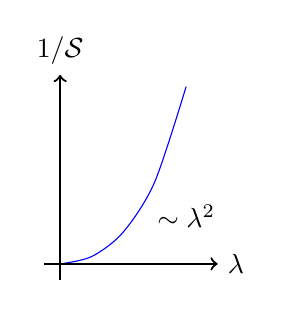
\begin{tikzpicture}[scale=2]
		\draw[blue, smooth] plot coordinates {(0,0) (0.2, 0.0464) (0.4,
		0.2011) (0.6, 0.5193) (0.8, 1.1259)};
		\draw[thick,->] (-0.1,0) -- (1, 0) node[right] {$\lambda$};
		\draw[thick,->] (0,-0.1) -- (0, 1.2) node[above] {$1/\mathcal{S}$};
		\draw (0.8, 0.3) node {$\sim \lambda^2$};
	\end{tikzpicture}
\end{center}
Large $\mathcal{S}$ implies small $\lambda$, i.e. small growth, and vice
versa. Note for water, $L/c_p \approx 80^{\circ}$C.

\subsubsection{Quasi-steady approximation}
When $\mathcal{S} \gg 1$ the Stefan condition implies growth is slow. Rescale
time $t \to \mathcal{S} t$ so the time derivative becomes
$\mathcal{O}(\mathcal{S}^{-1})$. Then
\begin{equation}
	\frac{\partial^2 T}{\partial x^2} \approx 0 \implies \frac{\partial
	T}{\partial x} = \frac{T_m - T_B}{a}
\end{equation}
i.e. there is a linear conduction profile in the solid. The Stefan condition
is now
\begin{equation}
	\rho L \dot{a} = k \left.\frac{\partial T}{\partial x} \right|_a \approx
	\frac{k(T_m - T_B)}{a}
\end{equation}
where $a = \sqrt{2\kappa t / \mathcal{S}}$. This definition of $a$ follows
from: $\mathcal{S} \gg 1 \implies \lambda \ll 1$. Then
\begin{equation}
	\sqrt{\pi} \lambda e^{\lambda^2} \erf \lambda = \frac{1}{\mathcal{S}}
	\approx \sqrt{\pi} \lambda \cdot 1 \cdot \frac{2}{\sqrt{\pi}} \lambda
\end{equation}
Hence $\lambda \sim (1/2\mathcal{S})^{1/2}$, from which $a(t) = 2\lambda
\sqrt{\kappa t}$ gives $a$ as above.

Note: as $t \to 0$, $\dot{a} \sim t^{-1/2} \to \infty$. This is physically
implausible; in fact growth is regularised by crystal kinetics which is not
included in this model.

\subsection{Phase change and fluid flow}
Consider 2D stagnation point flow driving a steady melting of a solid, with
fluid velocity
\begin{equation}
	\symbf{u} = (Ex, -Ez)
\end{equation}
\begin{center}
	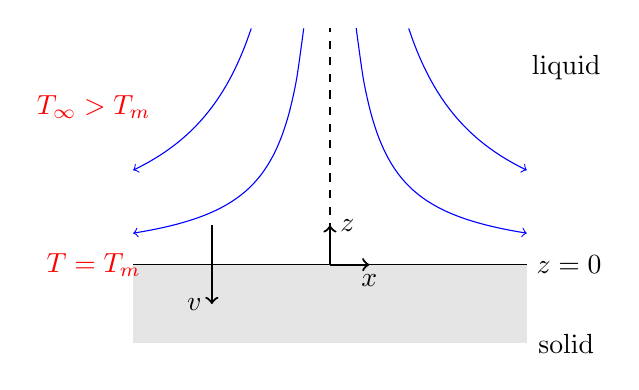
\begin{tikzpicture}
		\draw[draw=none,fill=gray!20] (0,0) rectangle (5, -1);
		\draw (0,0) -- (5,0) node[right] {$z=0$};
		\draw (5.5, 2.5) node {liquid};
		\draw (5.5, -1) node {solid};
		\draw[dashed] (2.5, 0) -- (2.5, 3);
		\draw[thick,->] (2.5,0) -- (3, 0) node[below] {$x$};
		\draw[thick,->] (2.5, 0) -- (2.5, 0.5) node[right] {$z$};
		\draw[thick,->] (1, 0.5) -- (1, -0.5) node[left] {$v$};
		\draw[red] (-0.5, 0) node {$T=T_m$};
		\draw[red] (-0.5, 2) node {$T_{\infty} > T_m$};
		\draw[blue,<-,smooth] plot[domain=0:2.167] ({\x},{-1/(\x-2.5)});
		\draw[blue,->,smooth] plot[domain=2.833:5] ({\x},{1/(\x-2.5)});
		\draw[blue,<-,smooth] plot[domain=0:1.5] ({\x},{-3/(\x-2.5)});
		\draw[blue,->,smooth] plot[domain=3.5:5] ({\x},{3/(\x-2.5)});
	\end{tikzpicture}
\end{center}

Steady-state in a translating frame of reference (i.e. moving with boundary at
speed $v$) implies $T = T(z)$ is a function of $z$ only. In steady-state are
left with a balance of advection and diffusion:
\begin{equation}
	(v-Ez)\frac{\partial T}{\partial z} = \kappa \frac{\partial^2 T}{\partial
	z^2}
\end{equation}
where $v$ is the melt rate. Neglecting advection by the frame (justify later)
we have solution
\begin{equation}
	T = T_m + (T_{\infty} - T_m) \erf \left( \sqrt{\frac{E}{2\kappa}} z \right)
\end{equation}
The Stefan condition gives
\begin{equation}
	-\rho L v = - k\left.\frac{\partial T}{\partial z} \right|_{z=0} = -k
	\frac{2}{\sqrt{\pi}} (T_\infty - T_m) \sqrt{\frac{E}{2\kappa}}
\end{equation}
Hence the melt rate can be written as
\begin{equation}
	v = \frac{1}{\mathcal{S}} \sqrt{\frac{2E \kappa}{\pi}}
\end{equation}

Note the following:
\begin{itemize}
	\item The melt rate $v$ increases as flow rate $E$ increases ($v \sim
		\sqrt{E}$)
	\item The thermal boundary layer has scale $\delta_T \sim \sqrt{\kappa/E}$.
		Thus $\delta_T$ decreases as $E$ increases, i.e. the flow compresses
		the thermal boundary layer
	\item The ratio of frame advection to flow compression is
		\begin{equation}
			\frac{\text{advection}}{\text{compression}} \sim \frac{v}{Ez} \sim
			\frac{v}{E\delta T} \sim \frac{v}{\sqrt{E\kappa}} \sim
			\frac{1}{\mathcal{S}}
		\end{equation}
		So neglect of frame advection is valid if $\mathcal{S} \gg 1$.
\end{itemize}

\subsection{Solidification with vigorous convection}
Consider solidification of a liquid with vigorous convection, so that there is
a well-mixed interior temperature $\overline{T}(t)$ in the liquid.
\begin{center}
	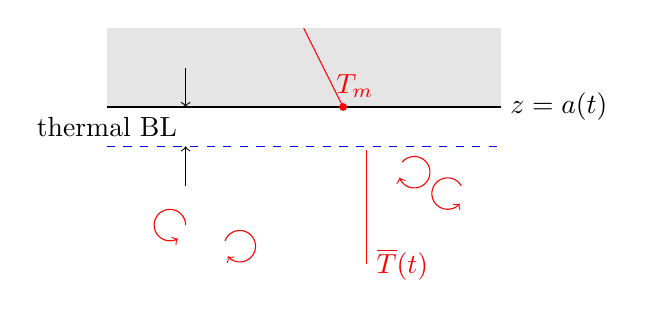
\begin{tikzpicture}
		\draw[draw=none,fill=gray!20] (0,0) rectangle (5, 1);
		\draw (0,0) -- (5, 0) node[right] {$z=a(t)$};
		\draw[dashed, blue] (0,-0.5) -- (5, -0.5);
		\draw[->] (1, 0.5) -- (1, 0);
		\draw[->] (1, -1) -- (1, -0.5);
		\draw (0, -0.25) node {thermal BL};
		\draw[fill=red,draw=none] (3, 0) circle (0.05);
		\draw[red] (3.15,0) node[above] {$T_m$};
		\draw[red] (3,0) -- (2.5, 1);
		\draw[red] (3.3, -0.55) -- (3.3, -2) node[right] {$\overline{T}(t)$};
		\draw[red,->] (1, -1.5) arc(0:300:0.2);
		\draw[red,->] (1.5, -1.7) arc (160:-140:0.2);
		\draw[red,->] (3.75, -0.7) arc (140:-160:0.2);
		\draw[red,->] (4.5, -1) arc (30:320:0.2);
	\end{tikzpicture}
\end{center}

Recall from earlier sections that high Rayleigh number convection has heat
flux
\begin{equation}
	F_T = \lambda k \left( \frac{\rho_0 g \alpha}{\kappa \mu}\right)^{1/3}
	\left( \overline{T} - T_m\right)^{4/3}
\end{equation}
Consider a control volume around the solid--liquid interface \emph{and} the
thermal boundary layer, and impose energy conservation. Note that the control
volume is in a frame of reference moving at the melt rate $v$ with the
interface.
\begin{center}
	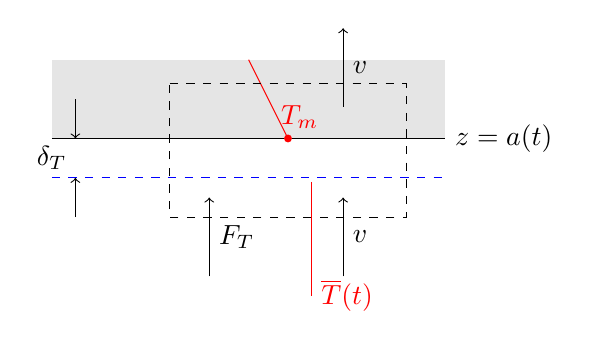
\begin{tikzpicture}
		\draw[draw=none,fill=gray!20] (0,0) rectangle (5, 1);
		\draw (0,0) -- (5, 0) node[right] {$z=a(t)$};
		\draw[dashed, blue] (0,-0.5) -- (5, -0.5);
		\draw[->] (0.3, 0.5) -- (0.3, 0);
		\draw[->] (0.3, -1) -- (0.3, -0.5);
		\draw (0, -0.25) node {$\delta_T$};
		\draw[fill=red,draw=none] (3, 0) circle (0.05);
		\draw[red] (3.15,0) node[above] {$T_m$};
		\draw[red] (3,0) -- (2.5, 1);
		\draw[red] (3.3, -0.55) -- (3.3, -2) node[right] {$\overline{T}(t)$};
		\draw[dashed] (1.5, 0.7) -- (4.5, 0.7) -- (4.5, -1) -- (1.5, -1) -- (1.5,
		0.7);
		\draw[->] (2, -1.75) -- (2, -0.75) node[midway,right] {$F_T$};
		\draw[->] (3.7, -1.75) -- (3.7, -0.75) node[midway,right] {$v$};
		\draw[->] (3.7, 0.4) -- (3.7, 1.4) node[midway,right] {$v$};
	\end{tikzpicture}
\end{center}

Conservation of energy with melt rate $v$ gives
\begin{equation}
	\rho (H_l - H_s)v + \rho c_p (\overline{T}-T_m)v + F_T - k \left.\frac{\partial
	T}{\partial z}\right|_{a^-} = 0
\end{equation}
Rearranging, we have
\begin{equation}
	\rho \left[ L + c_p(\overline{T}-T_m)\right] v = k \left.\frac{\partial
	T}{\partial z}\right|_{a^-} - F_T
\end{equation}
The first term is the release of latent heat, the second is cooling across the
boundary layer, the third is conduction in the solid and the final term is the
convective heat flux. This is the modified Stefan condition (needed for ES1
Q4).

\subsection{Earth's core}
Consider solidification of the Earth's inner core, driven by heat flux $F_m$
from the mantle. 

\begin{center}
	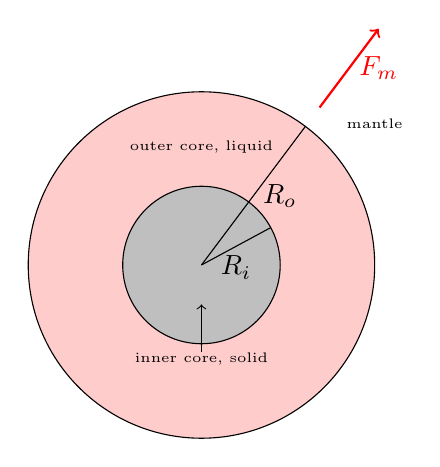
\begin{tikzpicture}
		\draw[fill=black] (0,0) circle (0.05);
		\draw[fill=red!20] (0,0) circle (2.2);
		\draw[fill=gray!50] (0,0) circle (1);
		\draw (0,0) -- (1.32,1.76) node[midway,right] {$R_o$};
		\draw (0,0) -- (0.88,0.475) node[midway,below] {$R_i$};
		\draw[red,thick,->] (1.5, 2) --++ (0.75,1) node[midway,right] {$F_m$};
		\draw (0, 1.5) node {\tiny outer core, liquid};
		\draw (0, -1.2) node {\tiny inner core, solid};
		\draw[->] (0, -1.1) -- (0, -0.5);
		\draw (2.2, 1.8) node {\tiny mantle};
	\end{tikzpicture}
\end{center}

We require a relation between the melt temperature $T_m = T_m(p)$ and the
pressure $p$, which is provided by the \emph{Clausius-Clapeyron equation}:
\begin{equation}
	\rho_s \frac{L}{T_m} \frac{\partial T_m}{\partial p} =
	\frac{\rho_s}{\rho_l} - 1
\end{equation}
The RHS quantity is position for iron in the inner core. To leading order, the
pressure is hydrostatic
\begin{align}
	\frac{\partial p}{\partial r} = - \rho g(r) &= - \rho \frac{G}{r^2} \left(
	\frac{4\pi}{3} r^3 \rho\right) = - \frac{4\pi}{3}G \rho^2 r \\
\implies p &= p_0 - \frac{2\pi}{3} G \rho^2 r^2
\end{align}
Substituting this form of the pressure into the Clausius-Clapeyron equation
gives
\begin{equation}
	T_m \approx T_0 - \frac{2\pi}{3} \frac{G T_0 (\rho_s - \rho_l)}{L} r^2
\end{equation}

The radius at which the core temperature $T$ is larger than $T_m$ is where the
solid--liquid interface exists, i.e. at $r=R_i$.
\begin{center}
	\begin{tikzpicture}[scale=3];
		\draw[thick,->] (-0.1, 0) -- (2.5, 0) node[right] {$r$};
		\draw[thick,->] (0, -0.1) -- (0, 1);
		\draw[red] plot[domain=0:2] ({\x},{1+1/(\x-3)});
		\draw[blue] plot[domain=0:1.667] ({\x},{1.2+1/(\x-2.5)});
		\draw[blue] (0,0.8) node[left] {$T_m$};
		\draw[red] (0,0.667) node[left] {$T$};
		\draw[dashed] (1.149,0.4597) -- (1.149, 0) node[below] {$R_i$};
	\end{tikzpicture}
\end{center}

Consider the two choices of limiting cases:
\begin{enumerate}
	\item No heat flux from inner core
	\item Perfectly conducting inner core $T_{IC} = T_m$. Outer core is
		convecting vigorously so assume well mixed, $T$ is adiabatic, i.e.
		`potential temperature' is isothermal.
\end{enumerate}

The balance of heat fluxes is
\begin{equation}
	4\pi R_0^2 F_m = \frac{4\pi}{3}\left[ R_0^3 - R_i^3\right] \rho c_p
	\frac{\partial T_m}{\partial t} + \rho L 4\pi R_i^2 \frac{\diffd
	R_i}{\diffd t}
\end{equation}
In case $(ii)$ the $R_i^3$ term in the first RHS term is neglected. In this
case,
\begin{equation}
	4\pi R_0^2 F_m = \frac{4\pi}{3} R_0^3 \rho c_p \cdot \frac{4\pi}{3}
	\frac{G T_m \delta \rho}{L} R_i \dot{R}_i + \rho L4\pi R_i^2 \dot{R}_i
\end{equation}
Hence the time averaged mantle heat flux is
\begin{equation}
	\frac{1}{m} \int_0^t F_m(t') \,\diffd t' = \zeta^2 + \mathcal{S} \zeta^3
\end{equation}
where $\zeta = R_i/R_o$, the Stefan number is $\mathcal{S} = \rho L R_o/m$ and
\begin{equation}
	m = \frac{2}{9} R_0^3 \rho c_p \frac{G T_m \delta \rho}{L}
\end{equation}
Real-world measurements give $\zeta = 1/3, \mathcal{S} = 0.4$, so growth is
controlled by the mantle heat flux balancing cooling (rather than latent
heat). Note that knowing $\zeta = 1/3$ does not allow a good estimate of the
age of the inner core, given the upper and lower bounds:
\begin{center}
	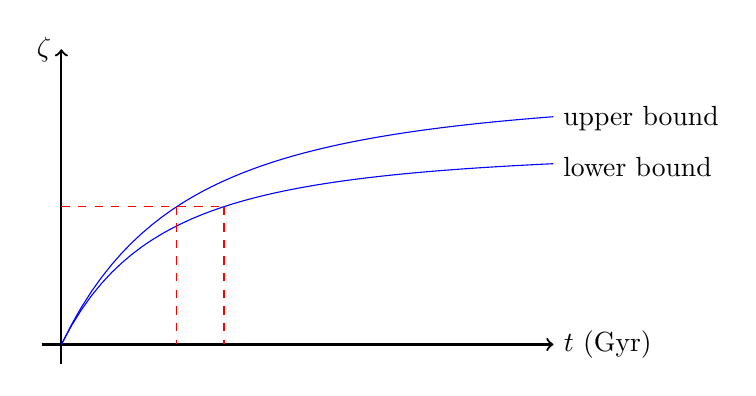
\begin{tikzpicture}[scale=2.5]
		\draw[thick,->] (-0.1, 0) -- (2.5, 0) node[right] {$t$ (Gyr)};
		\draw[thick,->] (0, -0.1) -- (0, 1.5) node[left] {$\zeta$};
		\draw[blue] plot[domain=0:2.5,samples=50] ({\x},{1-1/(\x+1)^2});
		\draw[blue] plot[domain=0:2.5,samples=50] ({\x},{1.3-2/(\x+1.24)^2});
		\draw (2.5, 1.15) node[right] {upper bound};
		\draw (2.5, 0.9) node[right] {lower bound};
		\draw[red,dashed] (0, 0.7) -- (0.826, 0.7);
		\draw[red,dashed] (0.826, 0.7) -- (0.826, 0);
		\draw[red,dashed] (0.586, 0.7) -- (0.586, 0);
	\end{tikzpicture}
\end{center}







\end{document}
